\section{\texorpdfstring{A k-matroid partíciós probléma -- MPP\textsubscript{$k$}}
		 {A k-matroid partíciós probléma}}

Adott $k$ darab $M_i = (E, F_i),$ ahol $i={\overline{1,k}}$ matroid. A kérdés,
hogy a matroidok összege ($\vee_{i=1}^{k}M_i$) a szabad matroidot ($E,2^E$)
adja--e? Másképp megfogalmazva előáll--e az alaphalmaz $E$ az $\cup_{i=1}^{k}
E_i$ alakban, ha $\forall i$-re $E_i \in F_i$. Feltehető, hogy az $E_i$ halmazok
diszjunktak, így egy partíciós problémához jutottunk.

\vspace{0.4cm}
\emph{MPP$_k$ P-beli probléma.}
\vspace{0.4cm}

MPP$_k \in$ NP, mert ha a feladatnak van megoldása, az egy tanú, amely lineáris időben
ellenőrizhető. MPP$_k \in$ coNP, mert ha a feladatnak nem létezik megoldása, akkor
adhatunk rá egy $X \subseteq E$ halmazt, ami biztosan összefüggő az összegben, azaz
$\sum r_i (X) < |X|$.

\subsection{Algoritmikus megoldás}

Most adunk erre egy algoritmust amely megoldja a feladatott, ehhez kiindul üres
halmazokból és addig bővíti azokat amíg uniójuk $E$ nem lesz. Ha egy adott
pontnál nem bővíthető tovább egyik halmaz sem, akkor az lesz a keresett ellenpélda,
ami bizonyítás arra, hogy a matroidok nem particionálhatók.

\begin{figure}[htbp]
\caption{Példa, hogy a mohó algoritmus miért nem működik:
		  $E_1 = \{2\}$, $E_2 = \{3\}$ állapotban nem tudunk újabb élt
		  belevenni egyik halmazba sem. Egy jó particionálás pedig a
		  $E_1 = \{ 1 \}$, $E_2 = \{ 2, 3 \}$ felosztás.}
\label{fig:MPPMohoNem}
\centering 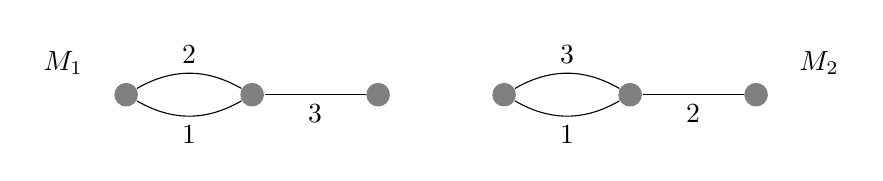
\begin{tikzpicture}[scale=0.8]
  \tikzset{ p/.style={circle,white,fill=gray,inner sep=0pt,minimum size=0.3cm},
  }
  \node[circle, fill=white] (M1) at (-3,0.5)   {$M_1$};
  \node[p] (1) at (-2,0)   {};
  \node[p] (2) at (0, 0)     {};
  \node[p] (3) at (+2,0)   {};

  \node[circle, fill=white] (M2) at (9,0.5)   {$M_2$};
  \node[p] (4) at (4,0)   {};
  \node[p] (5) at (6, 0)     {};
  \node[p] (6) at (8,0)   {};

  % the connection between the dots
  \draw[bend left,-]  (1) to node [midway, above] {$2$} (2);
  \draw[bend left,-]  (2) to node [midway, below] {$1$} (1);
  \draw[-]  (2) to node [midway, below] {$3	$} (3);

  \draw[bend left,-]  (4) to node [midway, above] {$3$} (5);
  \draw[bend left,-]  (5) to node [midway, below] {$1$} (4);
  \draw[-]  (5) to node [midway, below] {$2$} (6);
\end{tikzpicture}
\end{figure}

Az algoritmus egy $n+k$ pontú segédgráffal dolgozik ($|E|=n$ csúcs a halmazoknak
és $k$ csúcs a partícióknak), tehát $V' = E \cup \{p_1, p_2, \ldots, p_k\}$. A
gráf éleit definiáljuk, mint $(\overrightarrow{xy}) \in E'$ ahol:

\begin{figure}[htbp]
\caption{Segédgráf két halmazra}
\label{fig:MPP_graf}
\centering 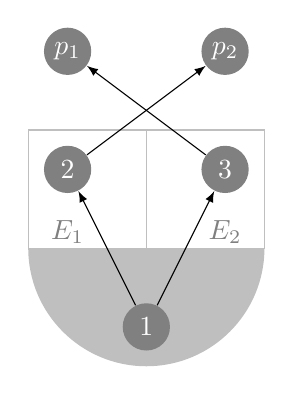
\begin{tikzpicture}[scale=1]
  \tikzset{ p/.style={circle,white,fill=gray,inner sep=0pt,minimum size=0.6cm},
  }
  \draw[lightgray] (0,0) rectangle(1.5,1.5);
  \draw[lightgray] (0,0) rectangle(-1.5,1.5);
  \node[circle,gray, fill=white] (E1) at (-1,0.2)   {$E_1$};
  \node[circle,gray, fill=white] (E2) at (+1,0.2)   {$E_2$};
  \path[fill=lightgray] (-1.5,0) arc [start angle=180, delta angle=180, radius=1.5];

  \node[p] (1) at (0,-1)   {$1$};
  \node[p] (2) at (-1,1)   {$2$};
  \node[p] (3) at (+1,1)   {$3$};
  \node[p] (p1) at (-1,2.5)   {$p_1$};
  \node[p] (p2) at (+1,2.5)   {$p_2$};

  \draw[-latex]  (1) -- (2);
  \draw[-latex]  (1) -- (3);
  \draw[-latex]  (2) -- (p2);
  \draw[-latex]  (3) -- (p1);

\end{tikzpicture}
\end{figure}


\begin{itemize}
  \item  $\begin{rcases}
  x \in E \\
  y = \{ p_i \}  \\
  x \not \in E_i\\
  E_i \cup  \{x\}  \in  F_i \end{rcases}
  \parbox[t]{11cm}{Egy ilyen él azt jelenti, hogy $x$-et hozzávehetjük $E_i$-hez
   a függetlenség megsérétése nélkül ($\overrightarrow{xp_i}$ -- az ábra felsõ
  részen a $p_i$-kbe mutató élek).}$
  \item $\begin{rcases}
  x,y \in E \\
  x \not\in E_i, y \in E_i\\
   E_i \cup \{x\} \not\in F_i,\\
   E_i \cup \{x\} - \{y\} \in F_i
  \end{rcases} \parbox[t]{10cm}{Egy ilyen él azt jelenti, hogy $x$-et
  hozzávehetjük $E_i$-hez, ha $y$-t elhagyjuk belöle ($\overrightarrow{xy}$ --
  az ábra alsó részén lévõ élek).}$
\end{itemize}

\begin{enumerate}
    \setcounter{enumi}{-1}
    \item $\forall~i~E_i = \emptyset$ kezdeti állapot ($i=\overline{1,n}$). Erre
    igaz, hogy $E_i \in F_i$.
    \item Keressük meg a legrövidebb irányított utat $E-\cup_{i}E_i$--ból
    $\left\{ p_1, \cdots, p_k \right\}$--ba.

    \item Ha létezik irányított út akkor ez meghatároz egy módosítás--sorozatot,
    hogy melyik $E_i$-t hogyan kell módosítanunk. Az út utolsó éle egy $p_j$-be
    megy, a többi $E$-beli elemek között, vagyis összesen 1-gyel növeljük
    $E_i$-k elem számát.  Ha egy {\it legrövidebb} ilyen út mentén javítunk,
    akkor bizonyítható, hogy $E_i$-k a módosítások után függetlenek maradnak (mi
    nem bizonyítjuk).
    \item Különben megállunk, nemleges a válasz, és a tanú $X$ az $E- \cup Ei$--ből
    irányított úton elérhető pontok halmaza.
\end{enumerate}

\begin{figure}[H]
\caption{Általános alakban}
\label{fig:MPP_halm}
\centering
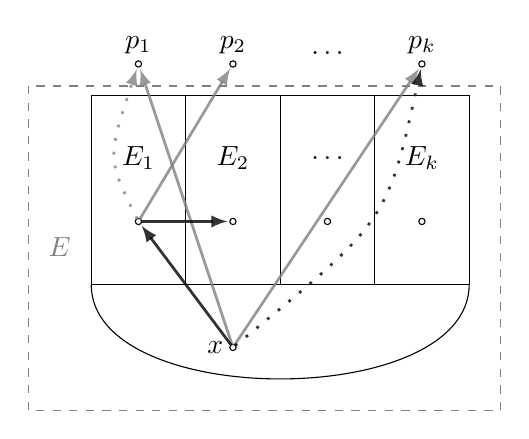
\begin{tikzpicture}[scale=0.8]
	\tikzstyle{vertex}=[draw,circle,fill=white,minimum size=3pt, inner sep=0pt]
 	\begin{scope}
		\draw (0,0) -- ++(6cm,0)
					-- ++(0,-3cm)
					-- ++(-6cm,0)
					-- (0,0);
		\foreach \x in {1,2,3} {
		\draw (\x*1.5,0) -- (\x*1.5,-3);
		}
		\draw (0.75,-1.0) node{$E_1$};
		\draw (2.25,-1.0) node{$E_2$};
		\draw (3.75,-1.0) node{$\dots$};
		\draw (5.25,-1.0) node{$E_k$};
		\draw (0,-3) .. controls (0,-5) and (6,-5) .. (6,-3);

		\draw (0.75, 0.5)  circle (0.5mm) node[above](1){$p_1$};
		\draw (2.25, 0.5)  circle (0.5mm) node[above](2){$p_2$};
		\draw (3.75, 0.5) node[above]{$\dots$};
		\draw (5.25, 0.5)  circle (0.5mm) node[above]{$p_k$};

		\draw (0.75, -2.0)  circle (0.5mm) node[left]{};
		\draw (2.25, -2.0)  circle (0.5mm) node[left]{};
		\draw (3.75, -2.0)  circle (0.5mm) node[left]{};
		\draw (5.25, -2.0)  circle (0.5mm) node[left]{};

		\draw (2.25, -4.0)  circle (0.5mm) node[left]{$x$};
		\draw[color=gray, dashed] (-1,0.15) rectangle (6.5,-5);
		\draw [color=gray] (-0.5,-2.4) node{$E$};
		\begin{scope}[opacity=0.8,>=latex]
			\draw (2.25, -4.0) [->, shorten >=2pt, shorten <=1pt, line width=1pt, color=gray] -- (0.75,0.5);
			\draw (2.25, -4.0) [->, shorten >=2pt, shorten <=1pt, line width=1pt, color=gray] -- (5.25,0.5);
			\draw (0.75, -2.0) [->, shorten >=2pt, shorten <=1pt, line width=1pt, color=gray, loosely dotted] .. controls (0.25,-	1) .. (0.75,0.5);
			\draw (0.75, -2.0) [->, shorten >=2pt, shorten <=1pt, line width=1pt, color=gray] -- (2.25,0.5);

			\draw (0.75, -2.0) [->, shorten >=2pt, shorten <=1pt, line width=1pt, color=black] -- (2.25,-2);
			\draw (2.25, -4.0) [->, shorten >=2pt, shorten <=1pt, line width=1pt, color=black] -- (0.75,-2);
			\draw (2.25, -4.0) [->, shorten >=2pt, shorten <=1pt, line width=1pt, color=black, loosely dotted] .. controls (4.7,-2) .. (5.25,0.5);

		\end{scope}
	\end{scope}
\end{tikzpicture}\end{figure}


\subsection{2-matroid-metszet probléma}

Adott $k$ matroid ($M_i=(E,F_i)$, ahol $i=\overline{1,k}$) és egy $p$ egész szám.
A kérdés, hogy létezik--e $F_i$--nek legalább $p$ méretű közös eleme?

Az így megfogalmazott probléma $k=2$--re MMP$_2$ komplexitása P--beli.
MPP$_k$--ra már beláttuk, hogy $P$--beli, MMP$_2$-őt pedig megfogalmazhatjuk
mint a $M_1 \vee M_2^*$ összeg szabad matroid--e?
